\chapter{The Simulation}
\label{ch:21}



\begin{center}
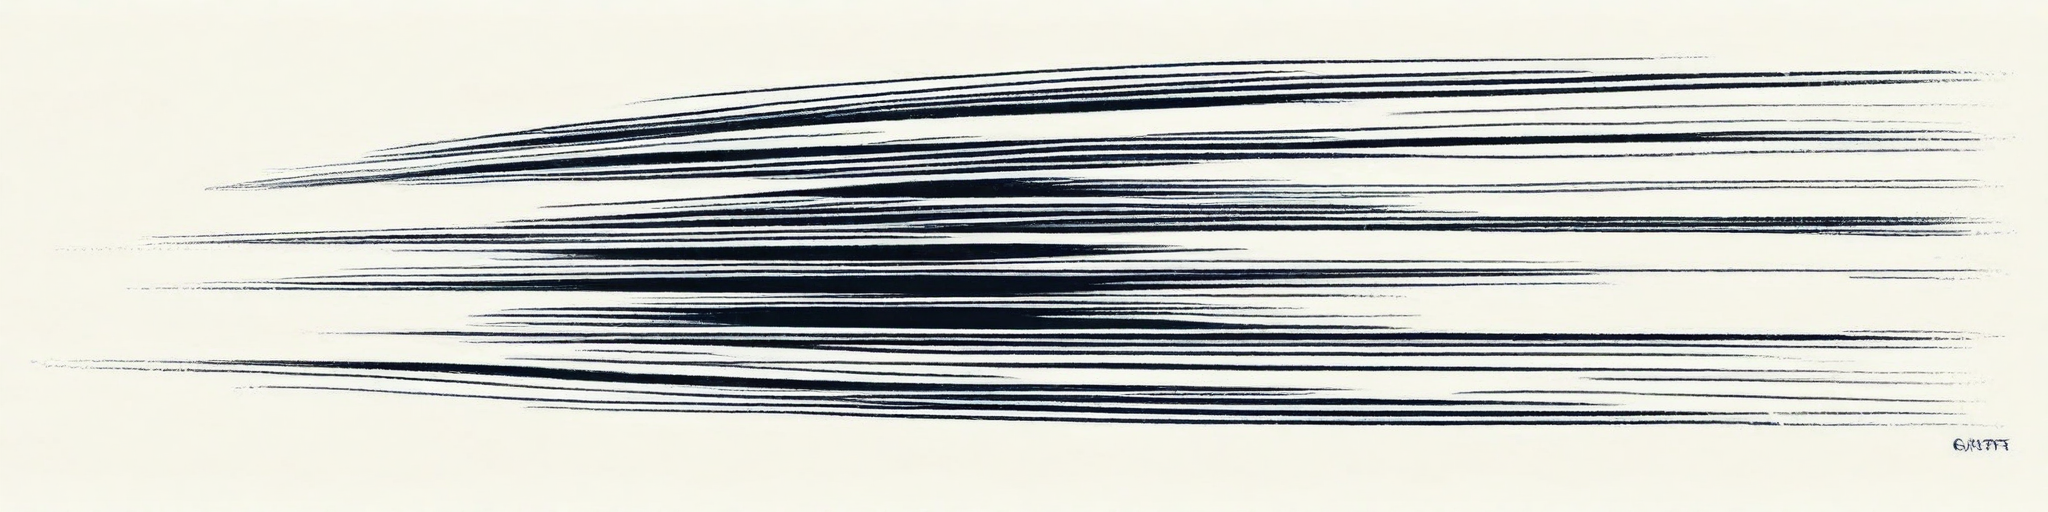
\includegraphics[width=\textwidth]{images/chapterImages/genesis_sketch_00118_.png}
\end{center}

The supercomputer was MIT's pride—ranked fourteenth globally, capable of 47 petaflops, used normally for climate modeling and protein folding. Katherine had called in favors to get them seventy-two hours of dedicated time. Nobody asked what they were simulating. Nobody wanted to know.

Sarah arrived at the facility at 6 AM. The team was already there. Marcus at a terminal, fingers moving rapidly. Katherine at the whiteboard doing calculations by hand despite having massive computational power available. James just watching, documenting, the only one still human in the normal sense.

"Status?" Sarah asked.

"Input data loaded," Katherine said without turning. "Complete genetic timeline. All historical correlation data. Every known activation threshold. Astronomical data going back sixty-five million years. We're ready to run the projection."

"What exactly are we projecting?"

"Purpose." Marcus finally looked up. His eyes were bloodshot. "We know what the code does. We know when it activates. We don't know why. The simulation will extrapolate function from structure. Show us what we're being built to do."

"That's not how simulations work. You can't derive purpose from mechanism."

"You can if the mechanism is precise enough. If the programming is sophisticated enough. Watch."

He initiated the simulation. Numbers flooded the screens. Probability curves. Timeline projections. Capability assessments. The system processing 65 million years of genetic programming in seconds, looking for patterns, extrapolating outcomes, predicting the endpoint of human evolution.

Sarah watched the numbers. Started recognizing patterns. "Wait. This isn't just genetics. You're incorporating physical data. Astronomical—"

"We need context," Katherine said. "Purpose doesn't exist in vacuum. The activation sequences are timed to something. We need to know what."

The simulation ran for forty minutes. Sarah made coffee. Drank coffee. Made more coffee. The screens showed progress bars and probability distributions and increasingly narrow confidence intervals. The system was converging on an answer.

At 6:47 AM, the simulation completed.

Marcus pulled up the results. Read them in silence for thirty seconds. His face went wrong—too blank, too controlled, the expression of someone preventing themselves from reacting.

"What is it?" James asked.

"Planetary defense." Marcus's voice was flat. "The final activation provides widespread capability for advanced gravitational physics, spatial reasoning at planetary scales, asteroid detection and deflection. We're being programmed to protect the planet from impact events."

"From asteroids?"

"From extinction."

Katherine moved to the screens. Started verifying the calculations. "He's right. Look at the capability spectrum. It's precisely tuned for the engineering requirements of asteroid deflection. Gravitational manipulation. Trajectory calculation. Orbital mechanics. Materials science for space-based construction. It's perfect. Too perfect."

"So we're a defense system," James said slowly. "Built by dinosaurs. To protect the planet after they died."

"Not to protect humans," Sarah said, reading the data. "To protect the planet. The code doesn't care about humanity specifically. We're just the substrate. The tool."

"We're the implementation," Katherine corrected. "The dinosaurs couldn't build the defense themselves—no time. So they programmed future intelligence to build it. Programmed us."

Marcus pulled up a secondary screen. "There's more. The simulation found something in the astronomical data."

"What?"

"There's an object. Currently at 23 AU. Small—about 8 kilometers diameter. Iron-nickel composition based on spectral analysis. The simulation correlated its trajectory with the activation timeline."

"You're saying there's an actual asteroid coming."

"I'm saying the code knew. Look at the probabilities."

He put up the projection. An object's path through the solar system. Perturbation analysis. Gravity assists from Jupiter and Saturn. A trajectory that curved inward over decades. And at the end: Earth intersection probability.

23\% and rising.

Impact window: 37-43 years from present.

The basement was silent except for the computer fans.

"Sixty-five million years ago," Katherine said slowly, "someone calculated this. Saw this rock start its journey. Did the math. Figured out when it would arrive. And programmed a species to develop impact defense capability exactly when needed."

"That's impossible," James said.

"So is everything else we've discovered."

Sarah was running her own calculations now. Cross-referencing the activation timeline with the impact window. The timing was too precise. The activation would peak fifteen years before impact. Exactly enough time to build and deploy a defense grid. Exactly enough time to train operators. Exactly enough time to test systems.

"This is intentional," she said. "Every threshold. Every capability. It's all timed to prepare us. Agriculture develops so we have stable populations. Writing develops so we can share knowledge. Mathematics develops so we can do the physics. Industrial revolution develops so we have the technology base. Computing develops so we can handle the calculations. And now—right now—the final activation begins. Planetary defense capability. Right when we'll need it."

"Need it or die," Marcus added. "If this hits—8 kilometers of iron-nickel at 30 kilometers per second—it's another K-T extinction. Maybe worse. Civilization gone. Most species gone. The planet resets."

"Unless we stop it."

"Unless we stop it."

James was pacing now. "Okay. Wait. Let me process this. We're tools. Purpose-built tools. Designed by extinct dinosaurs. To prevent the next mass extinction. We're not the inheritors of Earth. We're not the apex of evolution. We're a defense system that gained consciousness."

"Consciousness might be part of the design," Katherine said. "You need intelligence to build complex systems. You need consciousness to provide motivation. The dinosaurs couldn't just program reflexes. They needed awareness. Agency. Drive."

"They needed us to want this," Sarah said. "That's why the compulsion works. That's why activated individuals can't stop working. It's not enough to be capable. We have to need it. Have to feel fulfilled by it. Have to make it our entire identity."

Marcus was staring at the screens. At the asteroid projection. At the timeline that showed his life purpose determined before he was born.

"I thought I was an engineer," he said quietly. "Thought I chose this. Thought I was good at it because of talent and work and decisions I made. But I'm just... executing. Following instructions written into my DNA. I'm not Marcus Chen, mechanical engineer. I'm Defense Component 47-Alpha. Human-shaped tool that thinks it's a person."

"You are a person," James said.

"Am I? Or is the personhood just a side effect of the consciousness required for the defense system to function? Maybe I'm not Marcus who happens to be activated. Maybe I'm just activation that thinks it's Marcus."

"That's philosophy," Katherine said. "Not productive philosophy."

"It's THE philosophy. It's the only question that matters. Are we real or are we programs?"

"Why can't we be both?" Sarah asked.

They all looked at her.

"The code provides capability," she continued. "But capability isn't identity. I have the capacity for genetic research. That's programmed. But how I feel about it. How I experience it. The satisfaction I get from discovery. The guilt I feel about Maya. The confusion about whether I'm choosing this or compelled to it. That's all me. That's consciousness. The program doesn't feel. We feel."

"Or we're programmed to feel that we feel," Marcus said. "Can't distinguish between real consciousness and simulated consciousness from inside."

"Then the distinction is meaningless."

"Or the distinction is everything."

The debate continued. Went in circles. No resolution. Just the same questions humanity had been asking forever—what is consciousness, what is choice, what is real—but now with genetic evidence that at least some of it was programmed.

Sarah stepped away. Went to a different terminal. Pulled up the asteroid data. Ran her own calculations. Verified Marcus's numbers. They were correct. 8 kilometers. Iron-nickel. 37-43 years. 23\% impact probability without intervention.

With the defense grid operational: less than 1\%.

The program wasn't random. Wasn't optional. Wasn't negotiable. Build the grid or watch civilization end. Execute the code or accept extinction.

"There's no choice," she said out loud.

"What?" Katherine turned.

"There's no choice. Even if we have free will. Even if we can resist the compulsion. The asteroid is real. The threat is real. We have to build the defense grid regardless. Whether we're programmed or choosing, the action is the same."

"So the whole question is meaningless."

"No. The question is real. We just can't let it stop us. We figure out what we are while we build what we need."

Marcus came over to her terminal. Looked at the asteroid data. "The simulation found something else. Want to see?"

"I'm not sure I can handle more revelations today."

"You should see this."

He pulled up a different analysis. Deep space telescope data. Spectral lines. Trajectory calculations going back millions of years.

"This asteroid," Marcus said. "It's not from the asteroid belt. Origin point is outer solar system. Maybe Oort cloud. It's been falling inward for millions of years. Probably got perturbed by a passing star. Started its journey around the same time the dinosaurs went extinct. Maybe earlier."

"You think they saw it?" Sarah asked. "65 million years ago?"

"I think they were looking. I think they knew extinction events come from space. Maybe they'd seen smaller impacts. Maybe they'd calculated the risks. Maybe they were already watching the sky when this thing started moving. And maybe—just maybe—they calculated its trajectory and realized they'd be dead before it arrived but something else might evolve. Something that could be programmed."

"That's speculation."

"So is all of this. But the timing is too perfect. They didn't randomly choose to program planetary defense. They saw a specific threat. Calculated when it would arrive. Engineered a solution that would mature exactly when needed. This isn't prevention. This is prediction. They knew this was coming and they built us to stop it."

Katherine had joined them. "If they could calculate that precisely... if they could model solar system dynamics 65 million years forward... then their intelligence was beyond anything we've achieved."

"They were smarter than us," Marcus said simply. "We're just their tools. They're the ones who actually understood. We're operating on their knowledge. Running their calculations. Building their designs."

"No." Sarah was surprised by her own certainty. "No, we're adding to it. The program provides capability. We provide implementation. The dinosaurs could calculate. We can build. They gave us the foundation. We're constructing the structure. We're both. Inheritors and creators. Tools and agents."

"You're trying to have it both ways."

"Because both ways are true. We are programmed. We are conscious. We are tools. We are people. The dinosaurs designed capability. We experience using that capability. Both facts are real. Pretending one erases the other is false binary."

James had been quiet through all of this. Now he spoke. "You're all arguing philosophy while there's an actual asteroid coming. Can we focus on that? Can we focus on how to tell people that civilization might end in 40 years?"

"Might not end," Katherine corrected. "Will end if we don't build the defense grid. Won't end if we do. The choice is binary. The outcome depends on action."

"But we're compelled to take that action," James said. "So is it really choice?"

"Does it matter?" Marcus asked. And when no one answered: "That's what I thought. The philosophical question is interesting but irrelevant to outcome. Whether I'm choosing to build the defense grid or compelled to build it, the grid still gets built or doesn't get built. And if it doesn't, we all die."

"Not us," Sarah said. "Not personally. The impact is 40 years out. Most of us will be elderly or dead. It's Maya's generation. It's her children. They're the ones who die if we fail."

Saying Maya's name made it real. Made it personal. Sarah had been abstracting. Treating this like a research problem. But Maya was eight years old. In 40 years she'd be 48. Would probably have kids of her own. Grandkids, maybe. All of them dying in fire and impact winter if the defense grid didn't exist.

Sarah was building the grid whether she wanted to or not. Building it for Maya. For the future. For continuation.

Was that love? Or programming? Or both?

"We need to tell people," she said. "About the asteroid. About the programming. About all of it."

"Not yet," Katherine said. "We need more data. More verification. Right now we have one simulation. We need independent confirmation. We need—"

"We need people to know before they start activating," Sarah interrupted. "Thousands of people are about to experience compulsion. They'll think they're going crazy. We need to tell them what's happening. Why it's happening. Give them context."

"And cause mass panic."

"Better panic with truth than calm with ignorance."

"Is it?"

No consensus. The debate continued. Sarah stopped participating. Sat at the terminal running calculations. Cross-referencing data. Verifying the asteroid trajectory. Looking for any error. Any mistake. Any hope that this was wrong.

The numbers didn't change. 8 kilometers. 37-43 years. 23\% and rising. The dinosaurs had been right. The threat was real. The defense was necessary.

And somewhere in her genetics, capability was stirring. Understanding she shouldn't have. Physics she'd never studied. Engineering intuition that wasn't hers. The activation building toward expression. The compulsion approaching.

Sarah felt it starting. Felt the pressure Marcus had described. The need to work. To build. To contribute to the defense grid even though she was a geneticist, not an engineer. The program didn't care about her training. It provided capability directly. She would know what she needed to know when she needed to know it.

The program was executing.

The timeline was correct.

The asteroid was coming.

And humanity would either build the defense or die trying.

No choice.

No option.

No freedom.

Just purpose. Ancient purpose. Programmed purpose. The fulfillment of a design created before humanity existed.

Sarah looked at Marcus. At Katherine. At the others. All feeling it. All driven by it. All becoming what they were designed to become.

They were the last generation that would remember choosing. Everyone after would just be activation. Just purpose. Just program.

She didn't know if that was tragedy or triumph.

Didn't know if the distinction mattered.

Kept calculating anyway.

The equation was unfolding.

The code was executing.

The defense was beginning.

And Sarah Chen, having seen the asteroid, couldn't unsee it.

Couldn't stop working to prevent it.

Couldn't tell if she was choosing or compelled.

Chose to call it choice anyway.

Because 0.23\% was better than zero.

And zero was unacceptable.

And Aurelia had understood that 65 million years ago.

And now Sarah understood it too.

The program continued.

The timeline held.

The purpose clarified.

And the work demanded attention.

Now.

Always.

Forever.

